\documentclass{tufte-handout}

\title{Metodi di fluidodinamica computazionale CFD per una turbomacchina}

\author[Alberto Scomparin]{Alberto Scomparin}

%\date{28 March 2010} % without \date command, current date is supplied

%\geometry{showframe} % display margins for debugging page layout

\usepackage{graphicx} % allow embedded images
  \setkeys{Gin}{width=\linewidth,totalheight=\textheight,keepaspectratio}
  \graphicspath{{graphics/}} % set of paths to search for images
\usepackage{amsmath}  % extended mathematics
\usepackage{booktabs} % book-quality tables
\usepackage{units}    % non-stacked fractions and better unit spacing
\usepackage{multicol} % multiple column layout facilities
\usepackage{lipsum}   % filler text
\usepackage{fancyvrb} % extended verbatim environments
  \fvset{fontsize=\normalsize}% default font size for fancy-verbatim environments

\usepackage[italian]{babel}
\usepackage[T1]{fontenc}
\usepackage[utf8]{inputenc}

\usepackage{caption}
\usepackage{amsbsy}

% Standardize command font styles and environments
\newcommand{\doccmd}[1]{\texttt{\textbackslash#1}}% command name -- adds backslash automatically
\newcommand{\docopt}[1]{\ensuremath{\langle}\textrm{\textit{#1}}\ensuremath{\rangle}}% optional command argument
\newcommand{\docarg}[1]{\textrm{\textit{#1}}}% (required) command argument
\newcommand{\docenv}[1]{\textsf{#1}}% environment name
\newcommand{\docpkg}[1]{\texttt{#1}}% package name
\newcommand{\doccls}[1]{\texttt{#1}}% document class name
\newcommand{\docclsopt}[1]{\texttt{#1}}% document class option name
\newenvironment{docspec}{\begin{quote}\noindent}{\end{quote}}% command specification environment

% Notazione vettoriale
\newcommand{\vect}[1]{\pmb{#1}}
\newcommand{\de}[2]{\dfrac{\partial #1}{\partial #2}}
\newcommand{\dede}[2]{\dfrac{\partial^2 #1}{\partial #2^2}}

\begin{document}

\maketitle

\newpage

\tableofcontents

\newpage

\section{Introduzione}
\noindent
In questa relazione viene descritta la parte teorica e una possibile
implementazione in linguaggio Matlab del Metodo alle Differenze Finite \textsc{FDM}\marginnote{Finite Difference Method} e del Metodo degli Elementi Finiti \textsc{FEM}\marginnote{Finite Element Method}
per lo studio del campo di moto interno ad una turbomacchina.

Il fluido che scorre in una turbomacchina\footnote{\textbf{turbomàcchina}
s. f. (comp. di turbo- e macchina).
– Macchina motrice o operatrice a fluido, caratterizzata dalla presenza
di una ruota mobile calettata sull'albero della turbina
e munita alla periferia di pale che hanno la funzione di ricevere energia da
un fluido motore per trasmetterla all'albero
(turbomotrici), o anche quella
di trasmettere energia a un fluido, utilizzando il lavoro meccanico
che un motore fornisce all'albero della turbina (turbooperatrici).}
è un esempio di fluido-dinamica \emph{interna}: alcune delle condizioni al contorno 
del campo di moto sono date dall'impenetrabilità delle pareti del condotto; il sistema
risulta complessivamente chiuso, eccetto per entrata ed uscita del fluido.

\newpage

\section{Geometria del campo di moto}\label{sec:geometria}
\subsection{Semplificazione del dominio}\label{sec:turbomacchina}
La turbomacchina presa in esame è una pompa. Essa viene inizialmente modellata
come un corpo tridimensionale: il dominio del campo di moto è la porzione
di volume compresa all'interno della girante\footnote{Elemento rotante collegato all'albero
motore, in inglese \emph{impeller}}.
Il fluido per una pompa è un liquido, considerato incomprimibile.

\begin{figure}%
  \includegraphics[width=\linewidth]{pompa.png}
  \caption{Sezione di una pompa. La parte evidenziata in nero è la girante}
  \label{fig:pompa}
\end{figure}

Le pale della girante mettono in moto il liquido, ma non vengono considerate nel dominio
di riferimento. Vi sono vari modelli di pompe (e giranti) esistenti: in genere una variante 
del modello in figura.

\begin{figure}
    \centering
    \begin{minipage}{.3\textwidth}
      \centering
      \includegraphics[width=.9\linewidth]{impeller3d.png}
      \label{fig:impeller3d}
    \end{minipage}%
    \begin{minipage}{.6\textwidth}
      \centering
      \includegraphics[width=.9\linewidth]{impeller2d.png}
      \label{fig:impeller2d}
    \end{minipage}
    \caption{
        Sinistra: Modello CAD 3D di una girante.
        Destra: Sezione laterale di una girante, presa da [HuzHua1971].
        Si nota da subito la simmetria
    }
\end{figure}

Con una tale geometria il liquido entra in direzione 
assiale\footnote{$v_r = 0$} ed esce in direzione radiale\footnote{$v_z = 0$, se il condotto di uscita è sufficientemente lungo}, rispettivamente
su tutta la superficie di entrata ed uscita. Per informazioni sulla motivazione di tali imposizioni si
rimanda al brevetto\footnote{Ferdinand P. Sollinger, 1945 \textit{Centrifugal compressor entry vane}
\texttt{US2384265}}.

Siccome il fluido può soltanto entrare ed uscire attraverso le superfici menzionate,
la portata entrante ed uscente rimangono costanti e la \emph{continuità}\footnote{$\nabla\cdot\vect{V}=0$, per fluido incomprimibile} del fluido è assicurata.

% Figura girante da https://engineering.stackexchange.com/questions/2398/contours-of-radial-flow-impeller-vane
% Design of Liquid Propellant Rocket Engines, Huzel D., Huang D., NASA, 1971 p. 208
% Figura presa da http://my.fit.edu/~dkirk/4262/Liquid%20Rocket%20Engine%20Design.pdf 220 (208)

Una simmetria si manifesta lungo l'asse dell'albero motore: il campo fluido
è analizzabile sezionando il dominio con un semipiano generato a partire dall'asse di simmetria.
Ogni proprietà e geometria dei punti del dominio risultano
identiche\footnote{$\frac{\partial}{\partial\theta}=0 \quad \forall f(\vect{P}),\quad \vect{P} = (z,r,r\theta) $}
per qualsiasi angolo $\theta$.

Ci si pone allora in un sistema di riferimento cilindrico: scelto
un angolo $\theta$ arbitrario di sezione, il semipiano risultante è il dominio da studiare
divenuto bidimensionale in coordinate assiali $z$ e radiali $r$. L'ultima semplificazione impone
l'origine del sistema di riferimento nel punto dell'asse di simmetria all'entrata della
girante: il dominio è un solo quadrante\footnote{$z \geq 0, r \geq 0 $}.

\subsection{Nomenclatura}

Conviene stabilire una nomenclatura per ogni parte del dominio di cui si conoscono le
proprietà.

\begin{marginfigure}%
\centering
  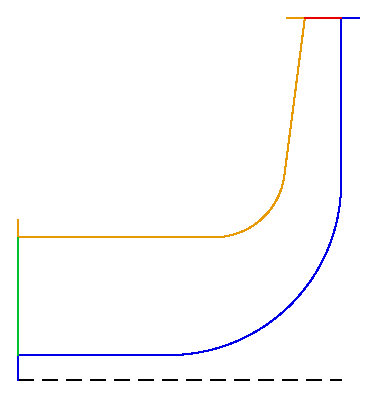
\includegraphics[width=.6\linewidth]{colori.eps}
  \caption{I colori indicano le superfici sezionate}
  \label{fig:colori2d}
\end{marginfigure}

Il \emph{mozzo} ha come parete la superficie di rotazione indicata in blu. Il mozzo è la porzione della girante calettata all'albero motore;
essendo una parete è considerata impenetrabile per il fluido.

La \emph{corona} ha come parete la superficie di rotazione indicata in arancione.
La corona è l'involucro che richiude la girante; impone al fluido la stessa condizione
del mozzo, con opportuno verso.

L'\emph{entrata} è la superficie - corona circolare - indicata in verde
dove entra il fluido; la velocità entrante è completamente assiale.

L'\emph{uscita} è la superficie - laterale di un cilindro - dove esce il fluido, la velocità
è completamente radiale se le pareti di mozzo e
corona sono perpendicolari all'asse di rotazione.

\begin{marginfigure}%
  \includegraphics[width=\linewidth]{entratauscita3d.png}
  \caption{La geometria delle superfici di entrata e uscita è evidente}
  \label{fig:entusc3d}
\end{marginfigure}

Anche se mozzo e corona rappresentano componenti reali tridimensionali della girante
si indica d'ora in poi come mozzo e corona le curve della figura \ref{fig:colori2d} 
con i rispettivi colori.
Ci si può ora liberare della complicata trattazione tridimensionale
concentrandosi sull'applicazione delle equazioni che regolano il moto del fluido
al dominio bidimensionale compreso tra i segmenti di entrata e uscita e le curve di mozzo
e corona.



\subsection{Implementazione del dominio}
Per implementare le equazioni del fluido è necessario avere una
parametrizzazione del dominio. Le dimensioni del dominio sono date dai parametri costruttivi
della girante.

Sarebbero sufficienti otto dati iniziali dai
quali si ricaverebbero in seguito i dodici\footnote{Sei punti a due coordinate ciascuno}
forniti in laboratorio.

A partire da queste coordinate la geometria del profilo si adatta
al variare dei parametri costruttivi.

\begin{marginfigure}%
  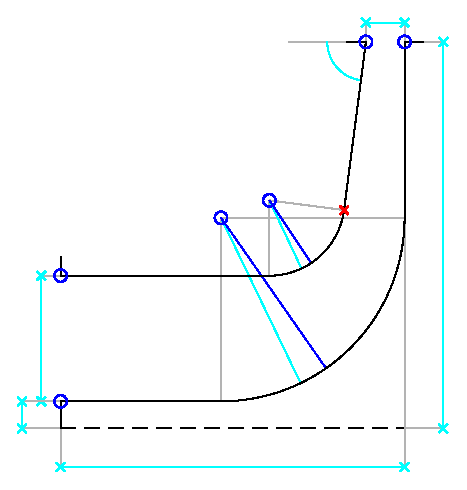
\includegraphics[width=\linewidth]{dimensioni.eps}
  \caption{In laboratorio vengono gentilmente fornite dal prof. Navarro le coordinate
    indicate in blu. Nell'implementazione sono richieste le coordinate dei punti in blu come dati iniziali}
  \label{fig:dimgirante}
\end{marginfigure}

Tali parametri iniziali potrebbero essere:
\begin{enumerate}
    \item Distanza dall'asse dell'entrata
    \item Lunghezza radiale dell'entrata
    \item Lunghezza assiale della girante
    \item Distanza dall'asse dell'uscita
    \item Lunghezza assiale dell'uscita
    \item Angolo uscita della corona
    \item Raggio di curvatura del mozzo
    \item Raggio di curvatura della corona
\end{enumerate}

Si suppone che la geometria sia quella di figura \ref{fig:impeller2d}, con l'angolo
di uscita del mozzo ortogonale all'asse di rotazione.
Si individuano i punti blu in figura \ref{fig:dimgirante}: i passaggi sono piuttosto semplici
e per semplicità si assumono direttamente note le coordinate dei punti. 

L'ascissa del punto all'entrata del mozzo, da cui si inizia a ricavare il resto dei punti,
è arbitraria e si pone uguale a \texttt{10}\footnote{Seguendo i dati forniti dal professore. Si può comunque considerare nulla e il risultato rimane inalterato}.
Altri punti notevoli sono quelli di inizio e fine curvatura di mozzo e corona

%%
% Codice Matlab da parametri geometrici a punti ovvi
%%

Il punto di tangenza nella corona tra la curvatura
e l'uscita rappresenta la complicazione maggiore per questa parte dell'implementazione.
Vi sono varie metodologie per individuarlo: si può risolvere un sistema tra il fascio di rette
passanti per il punto all'uscita della corona e la circonferenza contenente la curvatura della
corona.
In questa trattazione si sfruttano proprietà della geometria del dominio.

%% Figura a lato con angoli coincidenti

%%
% Codice Matlab per trovare punto di tangenza
%%

La parte fin'ora esposta è comune a entrambe le implementazioni.
I punti salvati nei vettori \texttt{zDominio} e \texttt{rDominio} servono per disegnare
facilmente il dominio del campo di moto. Tali punti non forniscono precisamente la forma
del campo in quanto sono discretizzazioni sufficienti a semplificare l'immagine di una curva
all'occhio.

Nel Metodo delle Differenze Divise la frontiera del dominio viene spezzata in funzioni definite
a tratti per discretizzare il dominio: all'occorrenza la funzione definita fornisce
$z=f_1(r),\ r=f_2(z)$.

Nel Metodo degli Elementi Finiti la frontiera viene parametrizzata invece come curva
definita a tratti con ascissa curvilinea.

%%%%%
% Legge campo moto
%%%%%

\newpage

\section{Legge del campo di moto}
La legge che regola il campo di moto è sostanzialmente espressa dalle equazioni di
continuità\footnote{$\frac{\partial \rho}{\partial t} + \nabla \cdot (\rho \vect{V})= 0$} e
di rotazionalità.
Dato che la pompa viene impiegata per dei liquidi, il fluido si può supporre incomprimibile
e l'equazione di continuità diviene la seguente, accompagnata dalla rotazionalità del campo fluido:
% Continuità
\begin{align}
    \nabla \cdot \vect{v} &= 0,
    \quad
    &\vect{v} = (v_{r}, v_{\theta}, v_{z})\\
    \nabla \times \vect{v} &= \vect{\omega},
    \quad
    &\vect{\omega} = (\Omega_r, \Omega_\theta, \Omega_z)
\end{align}
che in coordinate cilindriche\footnote{Anderson J. D., \emph{Fundamentals of Aerodynamics}, cap. 2} diventano:
\begin{equation*}
    \frac{1}{r}
    \de{(r \cdot v_r)}{r}
    +
    \frac{1}{r}
    \de{v_\theta}{\theta}
    +
    \de{v_z}{z}
    = 0
\end{equation*}
\begin{equation*}
    \left[
        \frac{1}{r}
        \de{v_z}{\theta}
        -\de{v_\theta}{z}
    \right]
    \cdot
    \vect{\hat{i}}_r
    +
    \left[
        \de{v_r}{z}-\de{v_z}{r}
    \right]
    \cdot
    \vect{\hat{i}}_{\theta}
    +
    \left[
        \frac{1}{r}
        \de{(r \cdot v_\theta)}{r}
        -
        \frac{1}{r}
        \de{v_r}{\theta}
    \right]
    \cdot
    \vect{\hat{i}}_z
    =
    \vect{\omega}
\end{equation*}
Per simmetria assiale si riducono a:
\begin{align}
    \frac{1}{r}
    \de{(r \cdot v_r)}{r}
    +
    \de{v_z}{z}
    &= 0 \label{eq:contass}
    \\
    \de{v_r}{z}
    -
    \de{v_z}{r}
    &=\Omega_\theta \label{eq:rotass}
\end{align}
Esse saranno il nucleo dell'equazione del moto che regola il campo fluido nel dominio. Per esaminare facilmente
il campo viene introdotta una funzione di corrente $\psi$, definita per un sistema di riferimento
assial-simmetrico nel piano meridiano come funzione di corrente di Stokes, dalla quale si ricava successivamente
in ogni punto del campo i valori di velocità $v(z,r)$ e pressione $p(z,r)$.

L'equazione \ref{eq:contass} si può esplicitare, con la derivata del prodotto, per la derivata parziale della velocità in $r$
o si può con essa evidenziare l'uguaglianza delle derivate parziali:
\begin{equation}
    \frac{\partial v_r}{\partial r}
    +
    \frac{v_r}{r}
    +
    \frac{\partial v_z}{\partial z} = 0,
    \quad
    \frac{\partial (r \cdot v_z)}{\partial z}
    =
    \frac{\partial (-r \cdot v_r)}{\partial r}
    \label{eq:contespl}
\end{equation}
La seconda delle precedenti esprime il fatto che la forma differenziale così definita:
\begin{equation}
    d\psi = (-r \cdot v_r) dz + (r \cdot v_z) dr
\end{equation}
è esatta\footnote{Una forma differenziale si dice esatta se in un dominio semplicemente connesso
le sue derivate in croce sono uguali tra loro}.
Questa si può scrivere anche come:
\begin{equation*}
    d\psi = \de{\psi}{z} dz + \de{\psi}{r} dr
\end{equation*}
Dove dunque $\psi$ è una funzione potenziale della forma differenziale.
Dalle due espressioni si ricavano le seguenti uguaglianze che legano velocità radiale e assiale alla funzione $\psi$:
\begin{equation}
    v_z = \frac{1}{r} \de{\psi}{r},
    \quad
    v_r = -\frac{1}{r} \de{\psi}{z}
    \label{eq:velcor}
\end{equation}

Preso un punto arbitrario $O$, che verrà considerato fisso, all'interno del dominio nel piano meridiano e un altro $P$ che si collega al primo con una curva semplice $\gamma$, la funzione $\psi$ si definisce perciò come:
\begin{equation*}
    \psi_P - \psi_O = \int_\gamma d\psi
    = \int_\gamma (-r \cdot v_r) dz + (r \cdot v_z) dr
\end{equation*}
Raccogliendo il prodotto scalare, si ottiene:
\begin{equation*}
    \int_\gamma (-r \cdot v_r) dz + (r \cdot v_z) dr
    = \int_\gamma r\cdot(v_z, v_r)\cdot (dr, -dz)
    = \int_\gamma r \cdot \vect{v} \cdot \vect{\hat{n}} ds
\end{equation*}
L'ultimo membro dell'equazione fornisce il senso fisico della funzione $\psi$: la portata di volume che attraversa la superficie aperta di rotazione della curva $\gamma$ arbitraria attorno all'asse di simmetria è data esattamente da $2\pi$ volte quel membro\footnote{Batchelor G. K., 1967, \emph{An introduction to Fluid Dynamics, p. 78}}.

La funzione di corrente $\psi$ rappresenta quindi sia il potenziale della forma differenziale data dall'equazione di continuità, sia la portata passante per la superficie di rotazione; la sua relazione con il vettore velocità $\vect{v}$ può essere riassunta nella formula della \emph{funzione di corrente di Stokes}:
\begin{equation*}
    \vect{v} = \nabla \times \frac{\psi}{r}  \cdot \vect{\hat{i}}_\theta
\end{equation*}

Il problema trattato in questa breve relazione concerne individuare la funzione $\psi$. Il sistema deve dunque essere ben posto: un'equazione regola l'andamento della funzione nel dominio e vigono le opportune condizioni al contorno.

Vi sono due tipi di condizioni al contorno, già accennate nella sezione \emph{Nomenclatura}, condizioni di Neumann, che sono vincoli alla derivata prima della funzione incognita, e di Dirichlet, vincoli al valore della funzione:
\begin{itemize}
    \item La frontiera all'entrata ha come condizione che la velocità radiale sia nulla:$\de{\psi}{z} = 0$
    \item La frontiera all'uscita
    virtuale\footnote{Parete di mozzo e corona devono essere ortogonali all'asse}
    ha come condizione che la velocità assiale sia nulla: $\de{\psi}{r} = 0$
    \item Si indica nella superficie del mozzo il valore percentuale di portata nullo $\psi = 0$
    \item Si indica nella superficie della corona il valore percentuale di portata totale $\psi = 100$
\end{itemize}
Note le condizioni al contorno, la legge da scegliere è tra le due espressioni \ref{eq:contass} e \ref{eq:rotass}.

Sostituendo nell'equazione di continuità \ref{eq:contass} le espressioni \ref{eq:velcor} delle velocità in relazione alla $\psi$ si ottiene:
\begin{equation}
    \dede{\psi}{r} - \frac{1}{r}\de{\psi}{r} + \dede{\psi}{z} = 0
    \label{eq:contpsi}
\end{equation}

Sostituendo nell'equazione di rotazionalità \ref{eq:rotass} le espressioni \ref{eq:velcor} delle velocità in relazione alla $\psi$ si ottiene, cambiando il segno dell'intera equazione:
\begin{equation}
    \de{}{z}\left(\frac{1}{r}\de{\psi}{z}\right)+\de{}{r}\left(\frac{1}{r}\de{\psi}{r}\right) = -\Omega_\theta
    \label{eq:rotasspsi}
\end{equation}

Nell'implementazione del Metodo delle Differenze Divise si approssimerà il valore di $\psi$ sfruttando la \ref{eq:contpsi} mentre in quella del Metodo degli Elementi Finiti si utilizzerà la \ref{eq:rotasspsi}.

\section{Metodo delle Differenze Divise}
% Discretizzazione dominio
\subsection{Discretizzazione del dominio}
La discretizzazione del dominio viene fatta dividendo la regione rettangolare che contiene l'intero dominio in rettangoli, la cui e distribuzione è scelta in base al numero di elementi richiesti. Conviene d'ora in poi tuttavia riferirsi ai nodi singoli e non ai rettangoli: il calcolo effettivo viene svolto in ogni nodo rispetto ai quattro adiacenti.
Nel caso della turbomacchina i nodi scelti in questa implementazione sono distinguibili essenzialmente in tre tipi: nodi interni, nodi al contorno, nodi esterni; un quarto tipo sono i nodi che non vengono considerati nel rettangolo di discretizzazione. La costruzione della griglia è stata progettata per avere i nodi coincidenti con punti della sezione all'ingresso e all'uscita (sui quali si applica necessariamente la condizione al contorno). Essendo mozzo e corona con parte curva la quadratura non coincide perfettamente: si prendono alcuni nodi esterni\footnote{Si veda in seguito} dove si può applicare con dovuti accorgimenti la condizione al contorno per lo svolgimento dell'iterazione.

% Espansione in serie di Taylor
\subsection{Derivata con notazione in serie di Taylor}
La legge del moto da risolvere è la \ref{eq:contpsi}. Compaiono in essa due derivate parziali del secondo ordine in due direzioni e una derivata parziale del primo ordine lungo $r$. Il metodo delle differenze divise consiste nell'applicare l'equazione di Laplace nei nodi discreti del dominio.
Si consideri una funzione $f(x)$ e la sua derivata nel punto $x$, definita come:
\begin{equation*}
    \de{f(x)}{x} =
    \lim_{\Delta x \to 0}
    \frac{f(x+\Delta x)-f(x)}{\Delta x}
\end{equation*}
Se si espande il termine $f(x+\Delta x)$ con serie di Taylor rispetto a $f(x)$, si ottiene:
\begin{equation*}
    f(x+\Delta x) = f(x) +
    \Delta x \de{f(x)}{x} +
    \frac{(\Delta x)^2}{2} \dede{u(x)}{x} + 
    o(\Delta x^3)
\end{equation*}
Dividendo e portando a primo membro:
\begin{equation*}
    \frac{f(x+\Delta x) - f(x)}{\Delta x} =
     \de{f(x)}{x} +
    \frac{\Delta x}{2} \dede{u(x)}{x} + 
    o(\Delta x^2)
\end{equation*}

Si può così scrivere un'espressione per $f$ in due punti, $f(x+\Delta x)$ e $f(x-\Delta x)$, note come rispettivamente differenza finita in avanti e all'indietro.
\begin{equation*}
    f_{i+1} = f_{i} + \Delta x \left(\de{f}{x}\right)_i + 
    \frac{(\Delta x)^2}{2} \dede{u(x)}{x} + 
    o(\Delta x^3)
\end{equation*}
\begin{equation*}
    f_{i-1} = f_{i} - \Delta x \left(\de{f}{x}\right)_i + 
    \frac{(\Delta x)^2}{2} \dede{u(x)}{x} + 
    o(\Delta x^3)
\end{equation*}

Sottraendo le due equazioni precedenti si ottiene un'espressione per la derivata \emph{centrale}:
\begin{equation}
    \left(\de{f}{x} \right)_i = \frac{f_{i+1}-f_{i-1}}{2\Delta x} + o(\Delta x^2)
    \label{eq:diffdiv1}
\end{equation}

Sommandole, invece, si ottiene un'espressione per la derivata del secondo ordine:
\begin{equation}
    \left(\dede{f}{x} \right)_i = \frac{f_{i+1}-2f_{i}+f_{i-1}}{\Delta x^2} + o(\Delta x^2)
    \label{eq:diffdiv2}
\end{equation}

% Legge con differenze divise
\subsection{Legge del moto con differenze divise}
La legge del moto con derivate parziali è esprimibile con differenze divise considerando le due direzioni $z$ e $r$ separatamente.

La legge non viene applicata nel dominio una volta sola nella sua interezza ma localmente a un nodo e ai quattro nodi ad esso adiacenti. Spostandosi di nodo in nodo si esegue nuovamente l'operazione fino ad arrivare ad una convergenza.

Si sostituiscono ora le espressioni \ref{eq:diffdiv1} e \ref{eq:diffdiv2} nella legge del moto; i pedici sono indicativi dei nodi con notazione in figura, con lo $0$ che indica il nodo su cui si calcola l'espressione:
\begin{fullwidth}
    \begin{align*}
        &\dede{\psi}{r} & &-\frac{1}{r}\de{\psi}{r} & &+ \dede{\psi}{z} &= 0 \\
        &\left(\dede{\psi}{r} \right)_0 &
        &-\frac{1}{r_0}\left(\de{\psi}{r} \right)_0 &
        &+\left(\dede{\psi}{z} \right)_0
        &= 0 \\
        &\frac{\psi_2-2\psi_0+\psi_4}{\Delta r^2} &
        &- \frac{1}{r_0} \frac{\psi_2-\psi_4}{2 \Delta r} &
        &+\frac{\psi_1-2\psi_0+\psi_3}{\Delta z^2}
        &=0
    \end{align*}
\end{fullwidth}

Estraendo dalle frazioni i vari valori di $\psi$:
\begin{fullwidth}
    \begin{equation*}
        -\psi_0\left[\frac{2}{\Delta r^2}+\frac{2}{\Delta r^2}\right]
        +\psi_1\left[\frac{1}{\Delta z^2}\right]
        +\psi_2\left[\frac{1}{\Delta r^2}-\frac{1}{2 r_0 \Delta r }\right]
        +\psi_3\left[\frac{1}{\Delta z^2}\right]
        +\psi_4\left[\frac{1}{\Delta r^2}-\frac{1}{2 r_0 \Delta r }\right]
        =0
    \end{equation*}
\end{fullwidth}

Siccome l'incognita è $\psi_0$, si isola dal resto:
\begin{fullwidth}
    \begin{equation}
        \psi_0 
        =
        \frac{\Delta r^2 \Delta z^2}{2(\Delta r^2 + \Delta z^2)}
        \left[
        \frac{\psi_1+\psi_3}{\Delta z^2}
        +\frac{\psi_2+\psi_4}{\Delta r^2}
        +\frac{\psi_2-\psi_4}{2 r_0 \Delta r}
        \right]
    \end{equation}
\end{fullwidth}

Se si considerano anche parametri di deformazione della differenza divisa per i nodi al contorno, l'equazione diventa:

\begin{fullwidth}
    \begin{equation}
        \psi_0 =
        \dfrac{
            \dfrac{
                \dfrac{\psi_2}{\lambda_2}
                +
                \dfrac{\psi_4}{\lambda_4}
            }
            {(\lambda_2+\lambda_4)\cdot \Delta r^2}
            +
            \dfrac{
                \dfrac{\psi_1}{\lambda_1}
                +
                \dfrac{\psi_3}{\lambda_3}
            }
            {(\lambda_1+\lambda_3)\cdot \Delta z^2}
            -
            \dfrac{
                \lambda_2 - \lambda_4
            }
            {
                2\cdot r_0 \cdot \Delta r \cdot (\lambda_2+\lambda_4)
            }
        }{
        \dfrac{
            \lambda_1 \cdot \lambda_3 \cdot \Delta z^2 +
            \lambda_2 \cdot \lambda_4 \cdot \Delta r^2
        }{
            \lambda_1 \cdot \lambda_2 \cdot \lambda_3 \cdot \lambda_4 \cdot \Delta r^2 \cdot \Delta z^2
        }
        }
    \end{equation}
\end{fullwidth}

Questa è l'equazione utilizzata nell'implementazione dell'algoritmo.\footnote{Si rimanda agli appunti delle lezioni per tutti i passaggi}
% Individuazione nodi
\subsection{Individuazione dei nodi}
Il criterio generale impiegato per scegliere i nodi si riassume nel seguente:

\emph{Se almeno un punto adiacente al nodo considerato è strettamente interno al dominio del campo di moto, allora il nodo viene incluso nella lista dei nodi}.

Questo criterio è stato scelto in modo che in ogni punto interno al campo di moto abbia un adiacente in ogni direzione e verso attraverso il quale calcolare la differenza divisa.

Per implementare la condizione sono stati parametrizzati mozzo e corona come funzioni in un piano $Oxy$ e i nodi della griglia come punti di tale piano.
Viene iterato ogni nodo della griglia a partire da quello con x e y minime incrementando prima verticalmente e poi orizzontalmente.
La condizione di controllo non viene effettuata sul nodo in sé ma sui punti di coordinate $x \pm \Delta x$ e $y \pm \Delta y$.
Se un punto adiacente si trova al di sopra della funzione mozzo e al di sotto della funzione corona allora il punto viene aggiunto alla lista con le sue coordinate $(z,r)$ rispettivamente date da $(x,y)$. 
Per velocizzare l'iterazione, se il nodo è al limite superiore del dominio si passa direttamente alla ascissa successiva.

Noti ora i punti da considerare, si imposta per i punti del mozzo il valore di $\psi$ a 0, per i punti della corona a 100 (si considera una funzione di corrente percentuale) mentre per i punti interni il valore medio 50 per velocizzare leggermente la convergenza.


% Individuazione adiacenti
\subsection{Individuazione dei nodi adiacenti ad ogni nodo}
Ora che si è in possesso della lista dei nodi necessari alla soluzione del campo fluido, è impostante metterli in relazione l'uno con l'altro, trovando i quattro nodi adiacenti ad ognuno.
I nodi adiacenti verticalmente sono semplici da trovare, in quanto la lista dei nodi viene fatta sequenzialmente in direzione r: i due adiacenti sono il precedente nella lista e il successivo.
Per gli adiacenti a destra e a sinistra si è scelto di partire dal nodo e di individuare andando per uno a ritroso e per l'altro in avanti il primo punto con la stessa ordinata del nodo. Così si sono ottenute per ogni nodo quattro liste, una per direzione, di nodi adiacenti.
Un accorgimento importante: se un nodo si trova al contorno verso una direzione, come nodo adiacente si sceglie il nodo stesso\footnote{In questo modo la differenza divisa lungo tale direzione, normale, risulta nulla e si ottiene la condizione di impermeabilità.}.

% Individuazione parametri di deformazione (lambda)
\subsection{Individuazione parametri di deformazione $\lambda$}
Per ovviare al problema della quadratura, si introducono dei coefficienti $\lambda$ che alterano lunghezza della differenza divisa in modo da riportare il nodo esterno precisamente al contorno e calcolare in modo più preciso la differenza divisa. Questo accorgimento risulta fondamentale per valori di $\Psi$ prossimi a 0 e 100. Per i punti interni al campo fluido il coefficiente per ogni direzione è banalmente 1, mentre per i punti al contorno di mozzo e corona va calcolato come la differenza tra la coordinata del nodo e la proiezione del nodo esterno sul contorno del dominio.

% Calcolo delle psi
\subsection{Linea di corrente}
Ora che tutti i parametri dell'equazione sono noti, si svolge l'iterazione. Come condizione si è scelto un numero massimo di iterazioni (per evitare calcoli eccessivamente lunghi) e contemporaneamente una tolleranza sulla differenza massima tra i nodi tra un'iterazione e la precedente (criterio di convergenza).

% Ricerca valori di psi a richiesta
Sono noti i valori di psi per ogni nodo della lista, si individuano i nodi che comprendono il valore cercato, e si prende il loro punto medio, rispettivamente in direzione verticale prima della curvatura, e orizzontale dopo la curvatura.

% Interpolazione valori con spline cubica
Note le coordinate dei punti cercati, essi vanno interpolati con una spline cubica per costruire una funzione che approssimi l'andamento della linea di corrente (che altro non è che una sezione della funzione di corrente).

% Possibili miglioramenti dell'algoritmo
\subsection{Miglioramenti possibili futuri}
Malgrado si sia cercato di rendere efficiente l'algoritmo di implementazione, per una maggiore chiarezza si è scelto di separare passaggi logici in operazioni diverse (ad esempio l'individuazione dei nodi e i loro adiacenti) mentre ne sarebbe potuta bastare una.
L'equazione risolutiva con i lambda è sufficiente impiegarla per i punti del contorno, mentre per quelli interni sarebbe più opportuno impiegare l'equazione semplificata.

Per una maggior precisione del valore di psi in uscita si sarebbe potuto estendere virtualmente il dominio fluido\footnote{Vedi Implementazione del Dominio} e tagliarlo successivamente una volta calcolate le $\psi$.

\section{Metodo degli Elementi Finiti}
% (Variazionale)
% \subsection{Metedo del variazionale con formulazione di Galerkin}
% Minimizzazione del variazionale tra funzione reale e funzione analitica.

%Equazione di Poisson integrale
% https://en.wikiversity.org/wiki/Introduction_to_finite_elements/Weak_form_of_Poisson_equation

% Integrazione equazione
\subsection{Equazione integrale}
Con le premesse date dalla formulazione del variazionale di Galerkin, è possibile trasformare l'equazione alle differenze \ref{eq:rotasspsi} nella seguente equazione integrale, detta formulazione debole dell'equazione di Poisson:
\begin{fullwidth}
\begin{equation}
     \iint_{D} G\de{}{z}\left(\frac{1}{r}\de{\psi}{z}\right) dr dz
    + \iint_{D} G\de{}{r}\left(\frac{1}{r}\de{\psi}{r}\right) dr dz
    = \iint_{D} -G\Omega_\theta dr dz
    \label{eq:intfem}
\end{equation}
\end{fullwidth}

% Interpolazione funzione psi con funzioni di forma distribuite nel dominio
% [https://academo.org/demos/3d-surface-plotter/?expression=1%2F4*(1-x)*(1-y)&xRange=-1%2C1&yRange=-1%2C1&resolution=39]
% Separazione equazione in sistema di equazioni
\subsection{Interpolazione della funzione incognita nel dominio}
L'equazione \ref{eq:intfem}, chiaramente, non è lineare: per risolverla è necessario dividere il dominio del profilo in elementi quadrilateri o triangolari; in questa trattazione è stato scelto l'impiego di elementi quadrilateri. Viene suddivisa in un sistema con tante equazioni quanti sono gli elementi isoparametrici e vale per ognuno di essi.
\begin{fullwidth}
\[\begin{cases}
    ...\\
     \iint_{D_j} \left[G\de{}{z}\left(\dfrac{1}{r}\de{\psi}{z}\right) 
    + G\de{}{r}\left(\dfrac{1}{r}\de{\psi}{r}\right)\right] dr dz
    = \iint_{D_j} -G\Omega_\theta dr dz \\
    ...
\end{cases}
\]
\end{fullwidth}

Tale suddivisione viene introdotta poiché non conoscendo i valori continui di $\psi$ la si interpola localmente nell'elemento con una \emph{funzione di forma}\footnote{La funzione di forma implementata permette di interpolare una funzione sommando quattro membri, ognuno dei quali rappresenta il peso unitario di ogni nodo, moltiplicati per il valore della $\psi_i$.}, in questo caso bidimensionale lineare. Per ricostruire la funzione, dunque, sono sufficienti i valori ai quattro vertici del quadrilatero della funzione $\psi_i,\ i = \{1,2,3,4\}$.

La funzione di forma impiegata è:
\begin{equation}
    N_i (\xi,\eta) = \frac{1}{4} \cdot (1+\xi \xi_i) \cdot (1+\eta \eta_i)
\end{equation}
La funzione $\psi$ viene interpolata nell'elemento j-esimo\footnote{Le coordinate non sono $z$ ed $r$, questa notazione vale infatti se si considera la funzione interpolata in un elemento \emph{parente}, ovvero quadrato centrato nell'origine di lato 2.} come:
\begin{equation}
    \psi = \sum_{i=1}^4 N_i (\xi,\eta)\cdot \psi_{k(i)}
    \label{eq:psiinterp}
\end{equation}\
Dove $k$ rappresenta l'indice del nodo rispetto all'intero dominio. Se l'elemento j-esimo ad esempio è formato dai nodi $k = \{2, 3, 8, 9\}$, ad essi corrispondono rispettivamente le funzioni di forma con indici $i = \{1, 4, 2, 3\}$\footnote{Fare riferimento alla figura per capire meglio la notazione indiciale}.

Sostituendo la funzione interpolata \ref{eq:psiinterp} nell'equazione integrale, e sfruttando la linearità dell'operatore di derivazione, il sistema si riassume nel seguente\footnote{Ricordando che la $N_i$ è definita in coordinate $\xi, \eta$}:
\begin{fullwidth}
\[\begin{cases}
    ...\\
     \sum_{i=1}^4 \psi_{k(i)}
     \iint_{D_j} \left[
        G\de{}{z}\left(\dfrac{1}{r}\de{N_i}{z}\right)
     +  G\de{}{r}\left(\dfrac{1}{r}\de{N_i}{r}\right)\right]
     dr dz
    = \iint_{D_j} -G\Omega_\theta dr dz \\
    ...
\end{cases}
\]
\end{fullwidth}

\subsection{Suddivisione del dominio nell'algoritmo}
Si è scelto di implementare le linee di mozzo e corona come curve parametriche con parametrizzazione ad ascissa curvilinea: in questo modo è possibile dividere il dominio in elementi con dimensioni pressoché similari.

\begin{marginfigure}%
  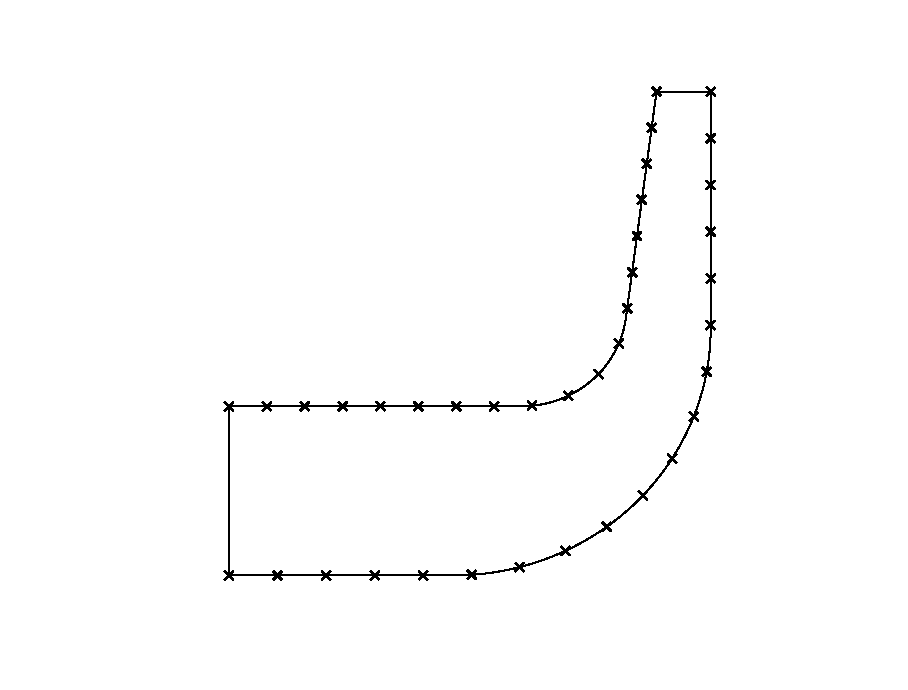
\includegraphics[width=\linewidth]{fem/divisione_lungo_moto.eps}
  \caption{Suddivisione longitudinale del dominio}
  \label{fig:divlung}
\end{marginfigure}

Lungo il moto si suddivide prendendo punti della curva con una frazione della lunghezza come parametro, ortogonalmente al moto si prendono i punti nella retta che passa tra l'i-esimo punto del mozzo e della corona, suddividendola a sua volta.

\begin{marginfigure}%
  \includegraphics[width=\linewidth]{fem/divisione_largo_moto.eps}
  \caption{Suddivisione in larghezza del dominio}
  \label{fig:divlarg}
\end{marginfigure}

Si ottengono matrici rettangolari di semplice ispezione: assegnate coordinate z e r si inseriscono i valori di \texttt{Psi} a \texttt{0} e \texttt{100} nella prima e ultima riga della matrice. Per i punti intermedi si è scelto il valore \texttt{NaN} (Not a Number), ma per lo scopo può andar bene anche \texttt{50} o altro valore qualsiasi purché diverso dai valori al contorno.

% Applicazione metodo di Green
\subsection{Applicazione del teorema di Green}
Grazie al teorema di Green (simile alla formula della derivata del prodotto) gli integrali a sinistra di ogni equazione si possono separare in componenti dovute all'interno del dominio e al contorno:
\begin{fullwidth}
\begin{equation*}
    g\de{f}{x}=\de{(g\cdot f)}{x} - \de{g}{x}\cdot f
\end{equation*}
\begin{align*}
    \iint_{D_j} \left[
        G\de{}{z}\left(\frac{1}{r}\de{\psi}{z}\right)
     +  G\de{}{r}\left(\frac{1}{r}\de{\psi}{r}\right)
    \right] dr dz
    &=
    \iint_{D_j} -G\Omega_\theta dr dz\\
    \iint_{D_j} \left[
        \de{}{z}\left(\frac{G}{r}\de{\psi}{z}\right)
        -\frac{1}{r}\de{G}{z}\de{\psi}{z}
        +\de{}{r}\left(\frac{G}{r}\de{\psi}{r}\right)
        -\frac{1}{r}\de{G}{r}\de{\psi}{r}
    \right] dr dz
    &=
    \iint_{D_j} -G\Omega_\theta dr dz
\end{align*}
Riordinando i termini con segno positivo:
\begin{equation*}
    \iint_{D_j} \left[
          \de{G}{z}\de{\psi}{z}
        + \de{G}{r}\de{\psi}{r}
    \right] \frac{dr dz}{r}
    =
    \iint_{D_j} \left[
          \de{}{z}\left(\frac{G}{r}\de{\psi}{z}\right)
        + \de{}{r}\left(\frac{G}{r}\de{\psi}{r}\right)
    \right] dr dz
    +
    \iint_{D_j} G\Omega_\theta dr dz
\end{equation*}
Applicando il teorema di Gauss-Green:
\begin{equation*}
    \iint_{D_j} \left[
          \de{G}{z}\de{\psi}{z}
        + \de{G}{r}\de{\psi}{r}
    \right] \frac{dr dz}{r}
    =
    \int_{\partial D_j}\frac{G}{r}\de{\psi}{z} (\hat{n}\cdot \hat{z})dr
    +
    \int_{\partial D_j}\frac{G}{r}\de{\psi}{r} (\hat{n}\cdot \hat{r})dz
    +
    \iint_{D_j} G\Omega_\theta dr dz
\end{equation*}
\end{fullwidth}
Dove il versore $\hat{n}$ indica la normale al contorno dell'elemento j-esimo diretta verso l'esterno.
% Applicazione metodo Galerkin
\subsection{Scelta della funzione di test}
Nella formulazione di Galerkin, la funzione di test è esattamente la funzione di forma riferita al nodo h-esimo $N_{i(h)}$. Per ogni equazione del sistema precedente ne esistono ora 4 date dai 4 nodi $h$ dell'elemento j-esimo. Mettendo assieme dunque tutte le considerazioni fin'ora esplicitate, si ottiene il sistema seguente:
\begin{fullwidth}
\[\begin{cases}
    ...\\
    \sum_{i=1}^4 \psi_{k(i)}
     \iint_{D_j} \left[
          \de{N_{i(h)}}{z}\de{N_{i(k(i))}}{z}
        + \de{N_{i(h)}}{r}\de{N_{i(k(i))}}{r}
    \right] \frac{dr dz}{r}= \\
    \qquad\qquad\qquad\qquad\qquad\qquad\qquad=
    \int_{\partial D_j}\frac{N_{i(h)}}{r}\de{\psi}{z} (\hat{n}\cdot \hat{z})dr
    +
    \int_{\partial D_j}\frac{N_{i(h)}}{r}\de{\psi}{r} (\hat{n}\cdot \hat{r})dz
    +\iint_{D_j} N_{i(h)}\Omega_\theta dr dz \\
    ...
\end{cases}
\]
\end{fullwidth}
La notazione degli indici può parere ridondante, ma è bene specificare il perché di tale notazione: la sommatoria è data dagli $i$ nodi che, se considerati con indici globali $k$, si possono considerare come nodi $k(i)$.

\begin{marginfigure}%
  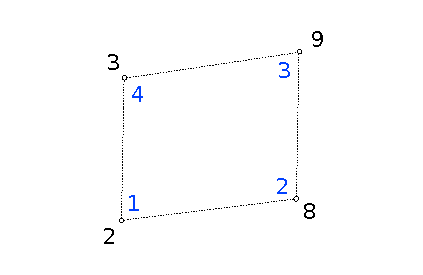
\includegraphics[width=\linewidth]{fem/indici_elemento.eps}
  \caption{In blu gli indici $i$, all'esterno gli indici con numerazione globale $k$}
  \label{fig:indici}
\end{marginfigure}

La funzione di forma è riferita ai nodi globali $k$, ma nelle coordinate locali $i$, dunque la funzione di forma si indica con $N_{i(k(i))}$ per esplicitare il fatto che è calcolata nell'elemento locale $j$ rispetto al nodo globale $k$, trovato cercando localmente gli $i$ vertici dell'elemento.

Dato che il nodo $h$ dell'equazione considerata non è dovuto alla sommatoria, la funzione di forma ad esso associato è soltanto $N_i(h)$.

Le funzioni di forma sono definite soltanto con l'indice $i = {1,2,3,4}$ e sono date dalle seguenti:
\begin{align*}
    N_1 &= \frac{1}{4}(1-\xi)(1-\eta)\\
    N_2 &= \frac{1}{4}(1+\xi)(1-\eta)\\
    N_3 &= \frac{1}{4}(1+\xi)(1+\eta)\\
    N_4 &= \frac{1}{4}(1-\xi)(1+\eta)
\end{align*}

\subsection{Contributi al contorno}
Ponendo attenzione al seguente termine:
\begin{equation*}
    \int_{\partial D_j}\frac{N_{i(h)}}{r}\de{\psi}{z} (\hat{n}\cdot \hat{z})dr
    +
    \int_{\partial D_j}\frac{N_{i(h)}}{r}\de{\psi}{r} (\hat{n}\cdot \hat{r})dz
\end{equation*}

il peso dato dalla $N_{i(h)}$ rende i contributi al contorno di ogni $D_j$ contenente il nodo $h$-esimo nulli una volta ricomposto il sistema, ad esclusione del contorno del dominio globale.

\begin{marginfigure}%
  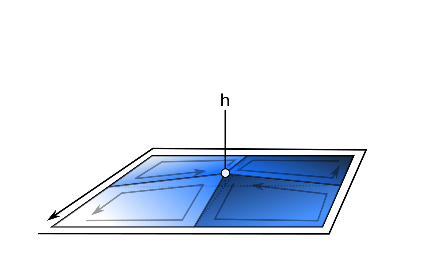
\includegraphics[width=\linewidth]{fem/contcontorno.eps}
  \caption{Una volta riassemblato il sistema, i contributi al contorno attorno al nodo h-esimo si elidono poiché sono uguali ma con direzione diversa; il contributo al contorno tra i 4 elementi è nullo perché nulla è la funzione di forma $N_{i(h)}$ nel tratto di percorso esterno}
  \label{fig:contcontorno}
\end{marginfigure}

Ciò può essere intuito anche dal fatto che il sistema stesso è stato costruito partendo dal considerare il dominio nella sua interezza. Siccome il teorema di Green vale anche se lo si considera nell'interezza, è naturale che il contributo del contorno debba essere dato soltanto dal contorno esterno.

Nel caso in cui il contorno dell'elemento sia effettivamente un contorno del dominio le condizioni al contorno del sistema (Neumann e Dirichlet) rendono questi contributi di frontiera nulli ugualmente:
\begin{itemize}
    \item {Dirichlet mozzo e corona: lungo il mozzo (e corona) è noto e costante il valore di $\psi$, percorrendo il contorno del mozzo (o della corona) entrambi i membri sono nulli poiché le derivate in entrambe le direzioni sono nulle.}
    \item {Neumann all'entrata: lungo l'entrata la velocità radiale è nulla, dunque il termine a destra si annulla}
    \item {Neumann all'uscita:  lungo l'uscita la velocità assiale è nulla, dunque il termine a destra si annulla}
    \item {Conservazione massa: dato che l'integrale delle velocità assiali lungo l'entrata e delle velocità radiali lungo l'uscita rappresenta l'intera portata del fluido, e che la normale è diretta in direzioni opposte (negativa per l'entrata e positiva per l'uscita), la continuità del moto annulla entrambe le componenti.}
\end{itemize}

\subsection{Introduzione coefficiente riassuntivo $a_{h,k}$}
Il sistema si riduce essenzialmente al seguente, dove l'equazione è la $h$-esima:
\begin{fullwidth}
\[\begin{cases}
    ...\\
    \sum_{i=1}^4 \psi_{k(i)}
     \iint_{D_j} \left[
          \de{N_{i(h)}}{z}\de{N_{i(k(i))}}{z}
        + \de{N_{i(h)}}{r}\de{N_{i(k(i))}}{r}
    \right] \dfrac{dr dz}{r}
    =
    \iint_{D_j} N_{i(h)}\Omega_\theta dr dz \\
    ...
\end{cases}
\]
\end{fullwidth}

Il temine integrale si può riassumere in un coefficiente, chiamato $a$:
\begin{fullwidth}
\begin{equation*}
    a_{h,k(i)}^J = 
    \iint_{D_j} \left[
          \de{N_{i(h)}}{z}\de{N_{i(k(i))}}{z}
        + \de{N_{i(h)}}{r}\de{N_{i(k(i))}}{r}
    \right] \frac{dr dz}{r}
\end{equation*}
\end{fullwidth}
Dove per $J$ si intende l'elemento $D_j$ e, dunque, il sistema diventa:
\begin{fullwidth}
\[
\begin{cases}
    ...\\
    \sum_{i=1}^4
    \psi_{k(i)}
    a_{h,k(i)}^J
    =
    \iint_{D_j} N_{i(h)}\Omega_\theta dr dz \\
    ...
\end{cases}
\]
\end{fullwidth}
Se si considera il moto irrotazionale (il che è ragionevole se non si presentano vortici o turbolenze nel campo di moto), la componente $\Omega_\theta$ si annulla e, espandendo la serie, il sistema risulta:
\begin{fullwidth}
\[
\begin{cases}
    ...\\
    \psi_{k(1)}
    a_{h,k(1)}^J
    +
    \psi_{k(2)}
    a_{h,k(2)}^J
    +
    \psi_{k(3)}
    a_{h,k(3)}^J
    +
    \psi_{k(4)}
    a_{h,k(4)}^J
    =
    0 \\
    ...
\end{cases}
\]
\end{fullwidth}
Ricapitolando, l'equazione indicata rappresenta l'equazione per il nodo $h$-esimo considerato appartenente all'elemento $j$-esimo e contando il contributo dei $k$ nodi dell'elemento.

Per risolvere l'integrale rappresentato da $a_{h,k}^j$ non si può procedere direttamente, poiché non sono note le derivate della funzione di forma in direzione $z$ ed $r$.
Sono però note le derivate in $\xi$ ed $\eta$:
\begin{equation}
    \de{N_i}{\xi}=\frac{\xi_i}{4}(1+\eta \eta_i) \qquad 
    \de{N_i}{\eta}=\frac{\eta_i}{4}(1+\xi \xi_i)
    \label{eq:defdforma}
\end{equation}

\begin{marginfigure}%
  \includegraphics[width=\linewidth]{fem/mappatura.eps}
  \caption{Come la funzione di forma permette di mappare un punto dalle coordinate $\xi,\eta$ nelle coordinate $r,z$, usando la \ref{eq:psiinterp} inserendo al posto di $\psi_{k(i)}$ i valori di $r$ e $z$}
  \label{fig:mappatura}
\end{marginfigure}

Nota la regola della catena, le derivate \ref{eq:defdforma} sono in relazione alle derivate nell'integrale come segue:
\begin{align*}
    \de{N_i}{\xi} &= \de{N_i}{z}\de{z}{\xi}+\de{N_i}{r}\de{r}{\xi} \\
    \de{N_i}{\eta} &= \de{N_i}{z}\de{z}{\eta}+\de{N_i}{r}\de{r}{\eta}
\end{align*}

\begin{fullwidth}
In notazione matriciale\footnote{La matrice in questa equazione è la matrice jacobiana di trasformazione dal dominio dell'elemento isoparametrico al dominio dell'elemento parente}:
\[
\begin{Bmatrix}
    \de{N_i}{\xi} \\ \de{N_i}{\eta}
\end{Bmatrix}
=
\begin{bmatrix}
    \de{z}{\xi} & \de{r}{\xi}\\ \de{z}{\eta} & \de{r}{\eta}
\end{bmatrix}
\begin{Bmatrix}
    \de{N_i}{z} \\ \de{N_i}{r}
\end{Bmatrix}
\]
\end{fullwidth}

Invertendo l'equazione:
\begin{fullwidth}
    \[
    \begin{Bmatrix}
        \de{N_i}{z} \\
        \de{N_i}{r}
    \end{Bmatrix}
    =
    \begin{bmatrix}
        \de{z}{\xi} & \de{r}{\xi}\\ \de{z}{\eta} & \de{r}{\eta}
    \end{bmatrix}^{-1}
    \begin{Bmatrix}
        \de{N_i}{\xi} \\ \de{N_i}{\eta}
    \end{Bmatrix}
    =
    \frac{1}{\de{z}{\xi}\de{r}{\eta}-\de{z}{\eta}\de{r}{\xi}}
    \begin{bmatrix}
        \de{r}{\eta}  &-\de{r}{\xi}\\ -\de{z}{\eta} & \de{z}{\xi}
    \end{bmatrix}
    \begin{Bmatrix}
        \de{N_i}{\xi} \\ \de{N_i}{\eta}
    \end{Bmatrix}
\]
\end{fullwidth}

Dato che sono note anche le derivate di $z$ e $r$ in $\xi$ ed $\eta$, si conoscono le $\de{N_i}{z}$ e $\de{N_i}{r}$ in funzione di $\xi$ ed $\eta$; devono inoltre essere noti anche i valori di $r_k$ e $z_k$ dell'elemento in cui si sta integrando.
Questo perché, ad esempio\footnote{Le altre sono facilmente ricavabili}:
\begin{equation*}
    \de{z}{\eta} = \sum_{i=1}^4 \frac{1}{4}\eta_i(1+ \xi \xi_i)z_{k(i)}
\end{equation*}

Non resta ora che parametrizzare il dominio dell'elemento isoparametrico secondo $\xi$ ed $\eta$. Per farlo è sufficiente la seguente uguaglianza:
\begin{equation*}
    dzdr = |\mathbb{J}|\ d\xi d\eta
\end{equation*}
L'integrale del coefficiente infine, diviene:
\begin{fullwidth}
\begin{equation*}
    a_{h,k(i)}^J = 
    \iint_{[-1,1]\times[-1,1]} \left[
          \de{N_{i(h)}}{z}(\xi,\eta) \de{N_{i(k(i))}}{z}(\xi,\eta)
        + \de{N_{i(h)}}{r}(\xi,\eta) \de{N_{i(k(i))}}{r}(\xi,\eta)
    \right] \dfrac{|\mathbb{J}(\xi, \eta)|}{r(\xi,\eta)} d\xi d\eta
\end{equation*}
\end{fullwidth}
Dove la distanza radiale $r$ è data dalla mappatura:
\begin{equation*}
    r(\xi,\eta) = \sum_{i=1}^4 \frac{1}{4} (1+\xi \xi_i)(1+\eta \eta_i) r_{k(i)}
\end{equation*}

Il coefficiente $a$ è ora integrabile con integrazione numerica, in particolare si usa in questa implementazione la quadratura di Legendre-Gauss:
\begin{fullwidth}
\begin{equation}
    a_{h,k(i)}^J \simeq 
    \sum_x \sum_y P_x \cdot P_y \left[
          \de{N_{i(h)}}{z}(\xi_x,\eta_y) \de{N_{i(k(i))}}{z}(\xi_x,\eta_y)
        + \de{N_{i(h)}}{r}(\xi_x,\eta_y) \de{N_{i(k(i))}}{r}(\xi_x,\eta_y)
    \right] \frac{|\mathbb{J}(\xi_x, \eta_y) |}{r(\xi_x,\eta_y)}
\end{equation}
\end{fullwidth}

La quadratura viene effettuata in particolari punti (a scelta, nell'implementazione sono stati usati 9 punti) cosiddetti di Legendre-Gauss. Per trovarli in una direzione o l'altra, vale la tabella seguente:

\begin{marginfigure}[15mm]%
  \includegraphics[width=\linewidth]{fem/mappatura_gauss.eps}
  \caption{L'integrazione viene effettuata nei 9 punti rimappati nel dominio di partenza}
  \label{fig:mappaturagauss}
\end{marginfigure}

\begin{center}
    \begin{tabular}{ c | c | c }
      n & j & $P_j$  \\ \hline
      1 & 0 & $2$ \\
      2 & $-\sqrt{\dfrac{1}{3}}$, $+\sqrt{\dfrac{1}{3}}$ & $1$, $1$\\
      3 & $-\sqrt{\dfrac{3}{5}}$, $0$, $+\sqrt{\dfrac{3}{5}}$ & $\dfrac{5}{9}$, $\dfrac{8}{9}$, $\dfrac{5}{9}$ 
    \end{tabular}
\end{center}



Scegliendo ad esempio 3 punti sia lungo la $\xi$ che la $\eta$ si ottengono 9 punti, così come implementato nell'algoritmo.

%%% MATRICE %%%%%%%%%%%
\subsection{Sistema lineare}
Ognuna delle $h$-equazioni può essere riassunta in un sistema lineare avente come matrice una matrice di coefficienti $a_{h,k(i)}$. Ogni nodo $h$ può avere da 1 a 4 elementi J di riferimento: per ogni equazione del sistema riferita al nodo $h$ si va a inserire una riga della matrice $\mathbb{A}$.

Ad esempio, se $h(1) = 2$, allora l'equazione del nodo 2 (globale) può ad esempio essere:
\begin{fullwidth}
    \begin{equation*}
        \psi_{1}
        a_{2,1}^{(1,7,8,2)}
        +
        \psi_{7}
        a_{2,7}^{(1,7,8,2)}
        +
        \psi_{8}
        a_{2,8}^{(1,7,8,2)}
        +
        \psi_{2}
        a_{2,2}^{(1,7,8,2)}
        =
        0
    \end{equation*}
\end{fullwidth}
Questa equazione vista come sistema con matrice è:
\begin{fullwidth}
    \[
        \begin{bmatrix}
            0					& 0 					& 0 					& \dots		& 0 		&	0					&	0					&	0	&	\dots & 0\\
a_{2,1}^{(1,7,8,2)} & a_{2,2}^{(1,7,8,2)} 	& 0  					& \dots		& 0 		& a_{2,7}^{(1,7,8,2)}	&	a_{2,8}^{(1,7,8,2)}	&	0	& 	\dots & 0\\
0					& 0 					& 0 					& \dots		& 0 		&	0					& 	0					&	0	& 	\dots & 0\\
\vdots				& \vdots 				& \vdots 				& \ddots	& \vdots 	&	\vdots				&	\vdots 				&	\vdots & \ddots& \vdots\\
0					& 0 					& 0 					& \dots  	& 0			&	0					&	0					&	0	& \dots & 0
        \end{bmatrix}
        \begin{Bmatrix}
            \psi_1       \\
            \psi_2       \\
            \vdots \\
            \psi_7 \\
            \psi_8 \\
            \vdots \\
            \psi_N       
            \end{Bmatrix}
        =
        \begin{Bmatrix}
            0       \\
            0       \\
            \vdots \\
            0       
        \end{Bmatrix}
    \]
\end{fullwidth}
Ricomponendo il sistema si riassumono i contributi, dati da ogni elemento j-esimo contenente il nodo h-esimo, nel solo coefficiente:
\begin{equation*}
    a_{h,k} = \sum_{j \in J_h} a_{h,k}^j, \quad J_h = J | \ h \in J
\end{equation*}

\begin{marginfigure}[-10mm]
    \centering
    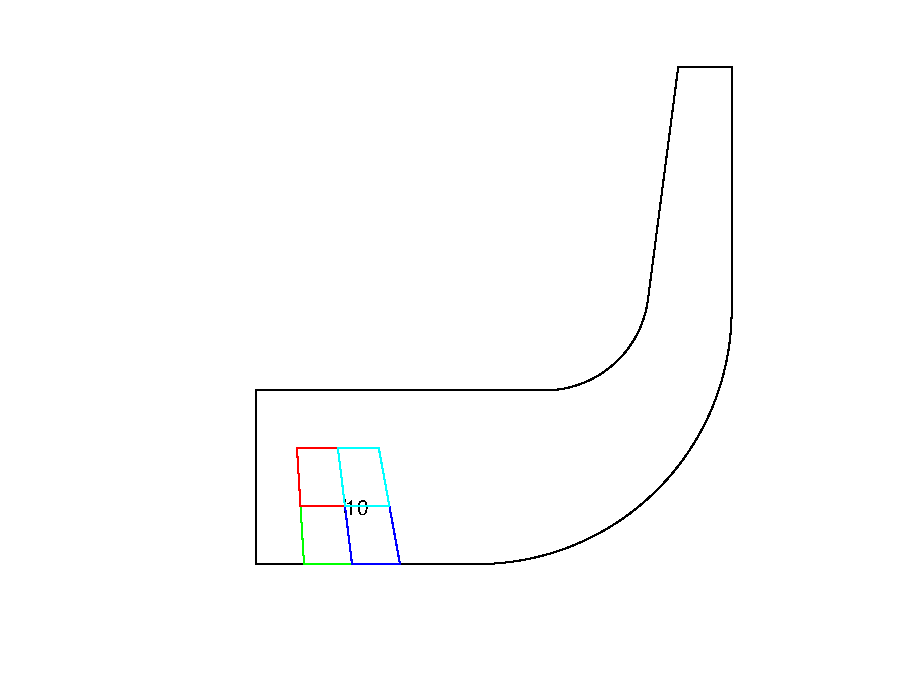
\includegraphics{fem/elementi_adiacenti.eps}
    \caption{Elementi adiacenti al nodo $h=10$}
    \label{fig:my_label}
\end{marginfigure}

Ove gli elementi $J_h$ sono gli elementi del dominio che contengono il nodo $h$ al loro interno. La matrice dell'intero sistema è riassumibile nella seguente:
\begin{fullwidth}
    \[
        \setcounter{MaxMatrixCols}{20}
        \begin{bmatrix}
        
           a_{1,1}   & a_{1,2} & 0          & \dots  & 0      & 0 & a_{1,i} & a_{1,i+1} & 0 & 0 & \dots  & 0 & 0 \\
a_{2,1}   & a_{2,2} & a_{2,3} & 0      & \dots  & 0              & a_{2,i}     & \ddots       & \ddots & 0      & \dots  & 0            & 0              \\
0            & a_{3,2} & a_{3,3} & \ddots & 0      & \dots          & 0              & \ddots       &        &        & \ddots & \vdots       & \vdots         \\
\vdots       & 0          & \ddots     & \ddots &        & \ddots         &                & 0            &        &        &        & 0            & 0              \\
0            & \vdots     & 0          &        &        &                &                &              & \ddots &        &        & \ddots       & 0              \\
0            & 0          & \vdots     & \ddots &        &                &                &              &        & 0      & \ddots & \ddots       & a_{N-i-1,N} \\
a_{i,1}   & a_{i,2} & 0          &        &        &                &                &              &        &        & 0      & a_{N-i, N-1}            & a_{N-i,N}   \\
a_{i+1,1} & \ddots     & \ddots     & 0      &        &                &                &              &        & \ddots & \vdots & 0            & 0              \\
0            & \ddots     &            &        & \ddots &                &                &              &        &        & 0      & \vdots       & 0              \\
0       & 0          &            &        &        & 0              &                & \ddots       &        &        &        & 0            & \vdots         \\
\vdots       & \vdots     & \ddots     &        &        & \ddots         & 0              & \dots        & 0      &        &        & \ddots       & 0              \\
0            & 0          & \dots      & 0      & \ddots & \ddots         & a_{N-1,N-i} & 0            & \dots  & 0      & \ddots & \ddots       & a_{N-1,N}   \\
0            & 0          & \dots      & 0      & 0      & a_{N,N-i-1} & a_{N,N-i}   & 0            & 0      & \dots  & 0      & a_{N,N-1} & a_{N,N}  
        \end{bmatrix}
        \begin{Bmatrix}
            \psi_1       \\
            \psi_2       \\
            \psi_3 \\
            \vdots \\
            \psi_{i} \\
            \psi_{i+1} \\
            \vdots \\
            \psi_{N-1} \\
            \psi_N       
            \end{Bmatrix}
        =
        \begin{Bmatrix}
            0       \\
            0       \\
            \vdots \\
            0       
        \end{Bmatrix}
    \]
\end{fullwidth}

L'indice $i$ dipende chiaramente da come si è suddiviso il dominio, e dall'ordine in cui si è scelto di procedere per numerare i nodi. Data la forma allungata del dominio, è consigliabile procedere numerando i nodi in direzione normale al moto, in modo che le fasce laterali alla diagonale siano più vicine alla diagonale\footnote{Dal punto di vista computazionale con una matrice così definita è più semplice risolvere il sistema.}.

Prima di risolvere il sistema bisogna calcolare i coefficienti $a_{h,k}$, poi ridurre il sistema portando a destra i nodi noti dalle condizioni di Dirichlet.

Si consideri la prima colonna della matrice $\mathbb{A}$: essa rappresenta il prodotto tra il coefficiente $a_{j,1}$ e il valore di $\psi_1$ in ogni riga $j$. Se il valore del nodo in questione è noto, si può portare a destra dell'equazione il prodotto tra $a$ e $\psi$ semplificando così il sistema: si elide la colonna, la riga riferita al nodo, e dunque anche la prima componente del vettore incognito $\vect{\Phi}$:
\begin{equation}
    [\mathbb{A}]\cdot\vect{\Phi}=\vect{0}
    \quad\to\quad
    [\mathbb{A}^{(1)}]\cdot\vect{\Phi}^{(1)}=-\vect{a}_1\cdot\phi_1 
\end{equation}
Questo procedimento viene iterato per tutti i nodi in cui viene imposta la condizione di Dirichlet, ottenendo il sistema finale ridotto:
\begin{equation*}
    [\mathbb{A}^{(p)}]\cdot\vect{\Phi}^{(p)}=\sum_{s\in MC}-\vect{a}_s\cdot\phi_s
\end{equation*}
L'insieme $MC$ rappresenta tutti i nodi facenti parte di mozzo e corona, e dunque il sistema da risolvere ridotto è un sistema di $N-p$ equazioni in $N-p$ incognite.
Risolto il sistema con un metodo computazionale a piacere sono noti tutti i valori di $\psi$ nei vertici di ogni elemento del dominio.
\subsection{Linea di corrente}
Per individuare le curve di livello della funzione di corrente $\psi$ bisogna impostare un valore di $\psi$ percentuale richiesto. In seguito bisogna individuare gli elementi del dominio che hanno tale valore compreso tra i quattro nodi ai vertici. Localmente si tratta semplicemente di ricavare $\eta$ in funzione di $\xi$ dall'equazione di interpolazione di $\psi$:
\begin{equation*}
    \psi_c = \sum_{i=1}^4 \frac{1}{4} (1+\xi \xi_i)(1+\eta \eta_i) \psi_{k(i)}
\end{equation*}
Esplicitando la sommatoria e saltando qualche passaggio si ottiene:
\begin{equation}
    \eta(\xi) = \frac{4 \psi_c - (1-\xi)(\psi_{k(1)}+\psi_{k(4)}) -(1+\xi)(\psi_{k(2)}+\psi_{k(3)})}
    {(1+\xi)(\psi_{k(3)}-\psi_{k(2)}) -(1-\xi)(\psi_{k(4)}+\psi_{k(1)})}
\end{equation}
Note le coordinate $\xi, \eta$ si possono rimappare $z, r$ per ottenere le coordinate dei punti nel dominio di partenza. Eseguendo l'operazione per tutti gli elementi contenenti il valore di $\psi$ cercato, si ottengono le linee di corrente.

\section{Risultati e confronti tra i metodi}
Come risulta chiaro dai grafici dei due casi, i metodi raggiungono risultati equivalenti se le suddivisioni del dominio sono sufficientemente elevate.

\begin{figure*}
    \centering
    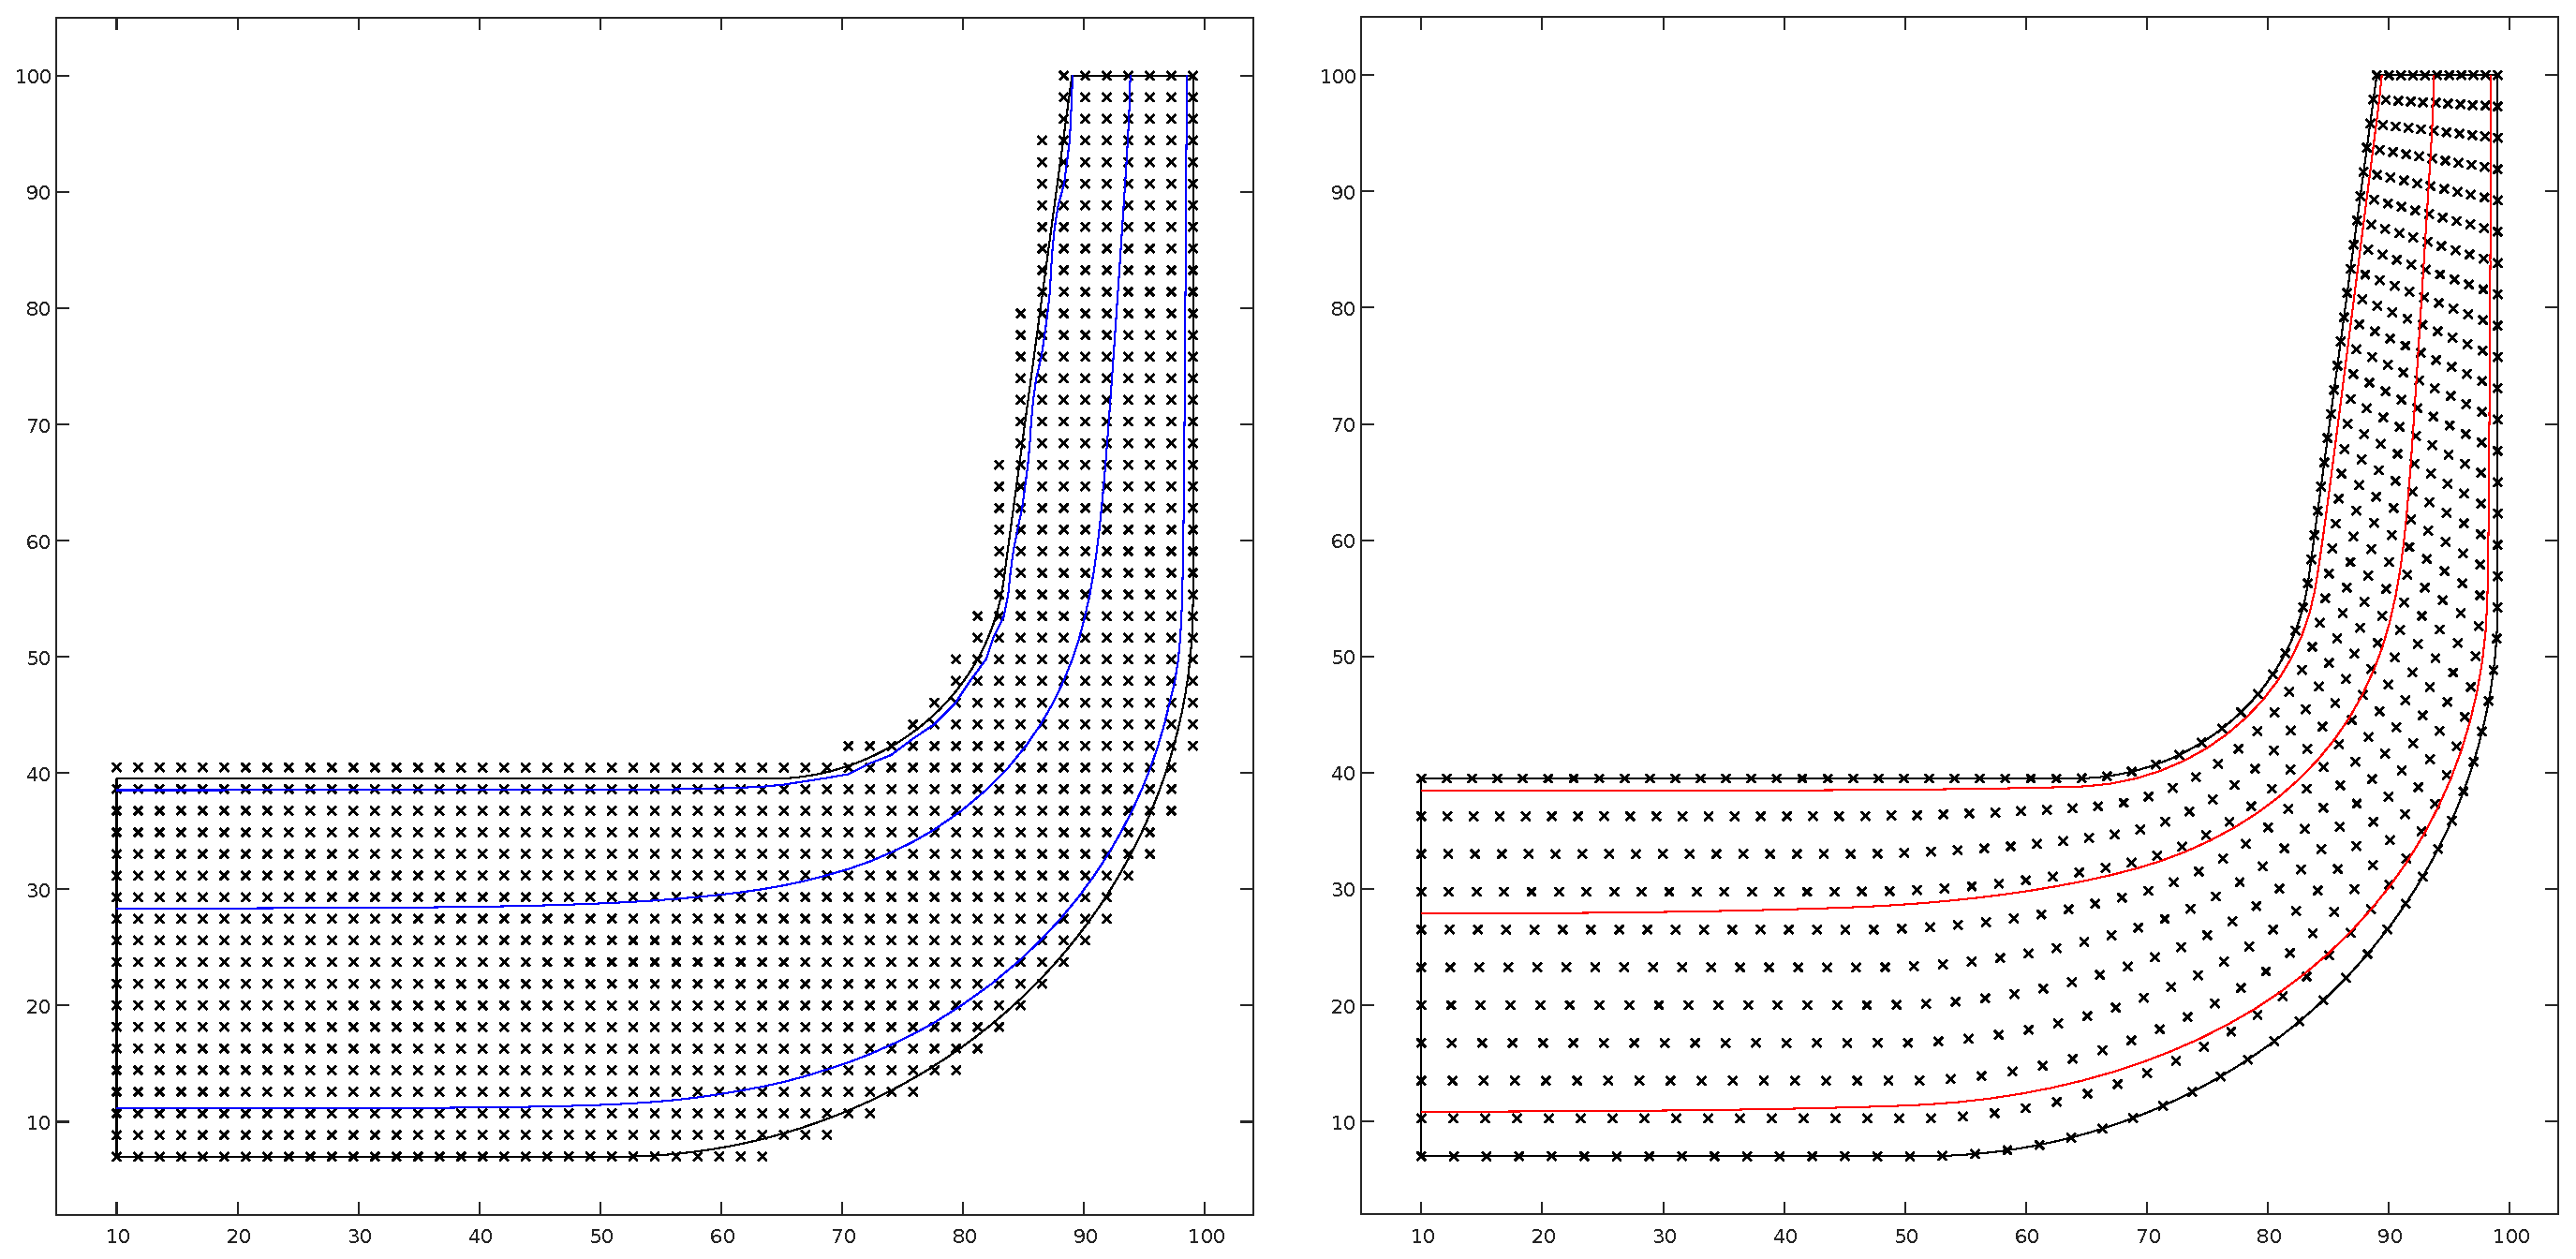
\includegraphics{fem_fdm_mesh.eps}
    \caption{Distribuzione dei nodi nei due casi: a sinistra la suddivisione è indipendente dalla forma del dominio: un numero di suddivisioni pari a 50 non è sufficiente (si osservi la linea di $\psi_{95}$); a destra  sono sufficienti poche suddivisioni che seguono il dominio per avere risultati soddisfacenti.}
    \label{fig:mesh}
\end{figure*}


\begin{figure*}
    \centering
    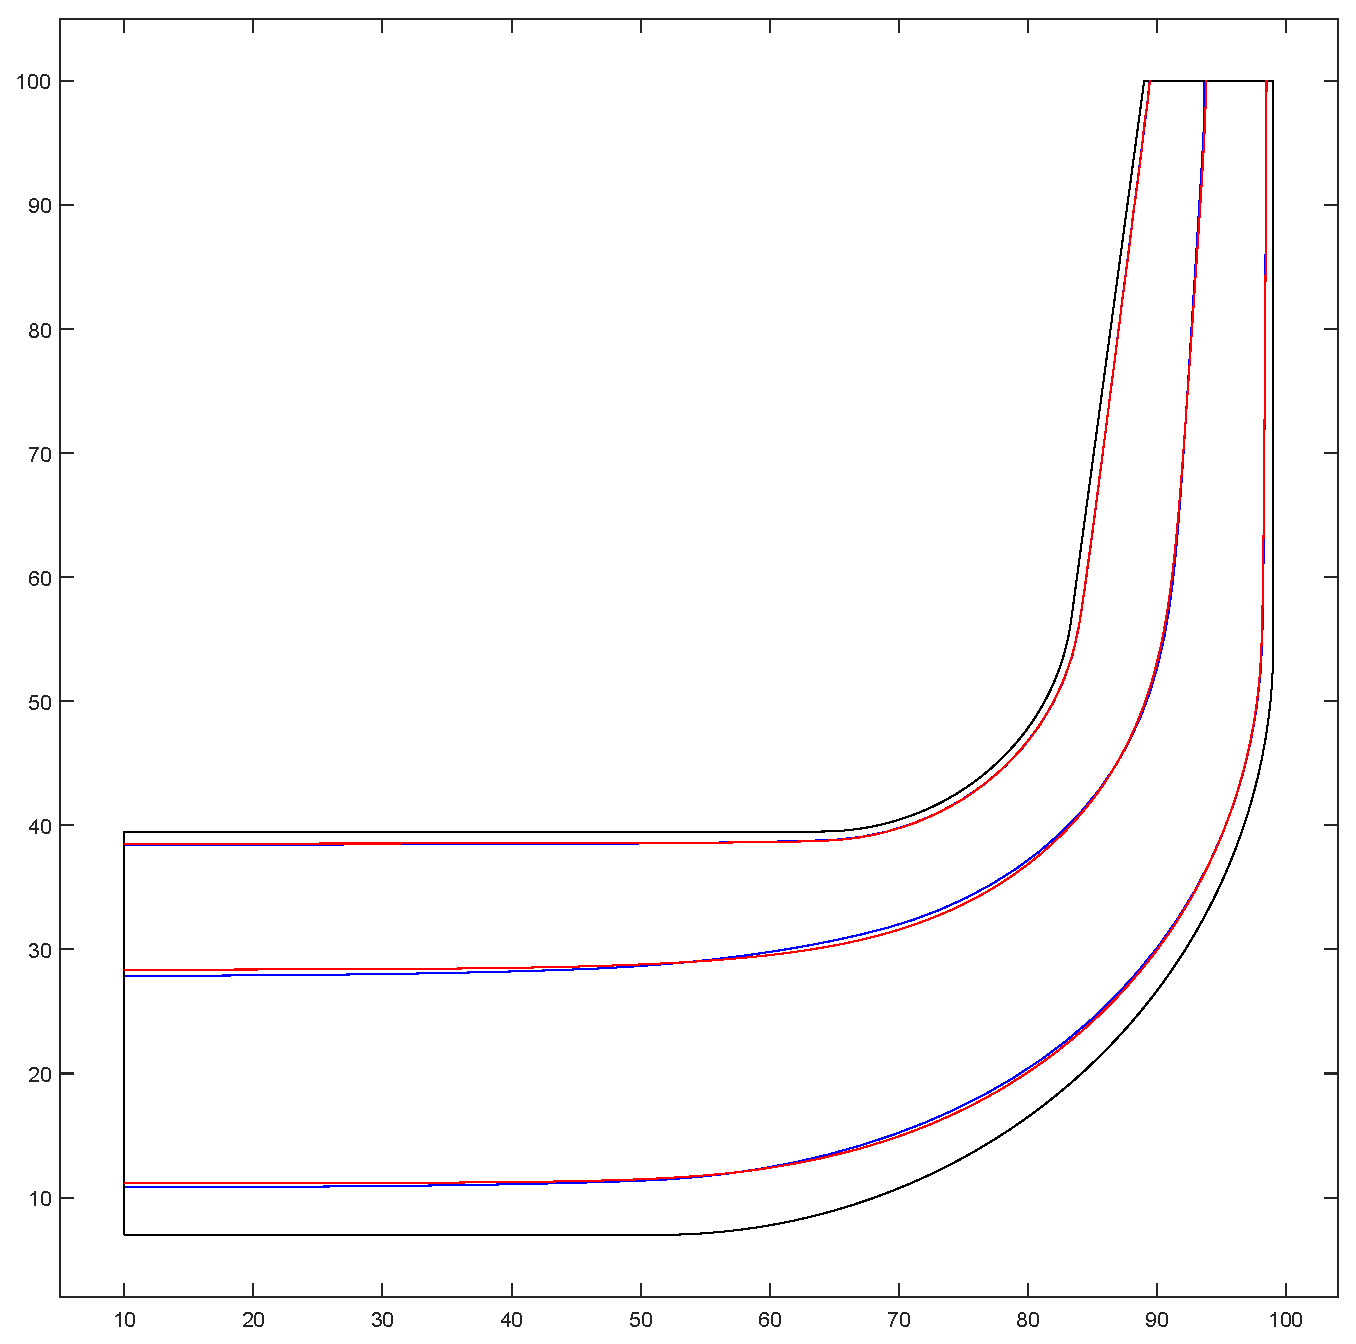
\includegraphics{fem_fdm_match.eps}
    \caption{Confronto tra i due risultati delle linee con $\psi$ percentuale ai valori di 5\%, 50\% e 95\%: in rosso Metodo degli Elementi Finiti, in blu Metodo delle Differenze Divise}
    \label{fig:match}
\end{figure*}

\end{document}